\documentclass[12pt, a4paper]{article}

\setlength{\headheight}{15pt}

\usepackage{float}
\usepackage[table,svgnames]{xcolor}

% Packages
\usepackage[english]{babel}
\usepackage{microtype}
\usepackage{amsmath,amsfonts,amsthm}
\usepackage{titling}
\usepackage{tikz}
\usetikzlibrary{positioning, calc, fit, arrows.meta}
\usepackage[hang, small, labelfont=bf, up, textfont=it]{caption}
\usepackage{array}
\usepackage{tabularx}
\usepackage{booktabs}
\usepackage{lastpage}
\usepackage{graphicx}
\usepackage{wrapfig}
\usepackage{enumitem}
\setlist{noitemsep}
\usepackage{hyperref}

% Margins
\usepackage{geometry}
\geometry{
    top=1.0cm,
    bottom=1.0cm,
    left=1.5cm,
    right=1.5cm,
    includehead,
    includefoot,
}

% Fonts
\usepackage[T1]{fontenc}
\usepackage[utf8]{inputenc}
\usepackage{XCharter}

% Headers and Footers
\usepackage{fancyhdr}
\pagestyle{fancy}
\renewcommand{\headrulewidth}{0.0pt}
\renewcommand{\footrulewidth}{0.4pt}
\lhead{}
\chead{\textit{KDP 2.0: Data Engineering Strategy}}
\rhead{}
\lfoot{}
\cfoot{}
\rfoot{\footnotesize Page \thepage\ of \pageref{LastPage}}

\fancypagestyle{firstpage}{
    \fancyhf{}
    \renewcommand{\footrulewidth}{0pt}
}

\title{KDP 2.0: Data Engineering Strategy}
\newcommand{\theothertitle}{Data Platform Integration, Hydration, and Operations}
\author{Matt Pappas, CDO}
\date{March 26, 2026}

\begin{document}

%----------------------------------------------------------------------------------------
% TITLE PAGE (HOUSE STYLE)
%----------------------------------------------------------------------------------------
\begin{center}
    \noindent\rule{\linewidth}{2pt}

    \vspace{0.5em}

    {\LARGE \bfseries \MakeUppercase{KDP 2.0: Data Engineering Strategy} \par}

    \vspace{0.25em}

    {\small Data Platform Integration, Hydration, and Operations}

    \vspace{0.5em}
    
    \noindent\rule{\linewidth}{2pt}

    \vspace{0.5em}

    \makebox[\linewidth][l]{%
      \begin{tabular}{@{} l @{}}
        \textbf{Author:} Matt Pappas, CDO \\ [6pt]
        \textbf{Date:} March 26, 2026
      \end{tabular}%
    }

    \vspace{0.5em}

    \noindent\rule{\linewidth}{2pt}
\end{center}

\setcounter{page}{1}
\thispagestyle{firstpage}

\section{Introduction}

\subsection{Scope}
This paper outlines how \textbf{Data Engineering} will be built on the Kiewit Data Platform (KDP). Specifically:
\begin{itemize}
    \item Building the Kiewit Data Platform 2.0
    \item Care and feeding of the platform (operations, monitoring, optimization)
    \item Executing the data projects outlined through the Kiewit Intelligence Program (KIP) via Data Strategy
\end{itemize}

\noindent This paper does \textbf{not} cover:
\begin{itemize}
    \item Data Strategy (architecture, domain planning, governance)
    \item Web Development
    \item Data Science (modeling, ML, analytics)
\end{itemize}

\subsection{Author's Recommendation}
It remains the recommendation of the author to keep Data Engineering and Data Science within one organization. Separation creates:
\begin{itemize}
    \item Unintegrated data pipelines
    \item Data sprawl (28+ Snowflake databases today)
    \item Data complexity—the silent killer of velocity
    \item Data architecture cannot engage effectively when 25+ person groups build pipelines differently—standardization is a prerequisite for governance.
\end{itemize}

\section{The Problem}
Kiewit data teams cannot deliver data science or data products at the velocity Kiewit needs. The root cause is organizational structure.

\subsection{KIP Objectives (What We Need)}
These objectives were established through multiple strategy documents:
\begin{itemize}
    \item \textit{Reorganizing Data Science and Engineering Teams for Efficiency and Throughput} (August 2025)
    \item \textit{Caterpillar Helios: Next-Generation Data Orchestration Platform} (September 2025)
    \item \textit{Kiewit Intelligence Platform: Executive Summary} (November 2025)
    \item \textit{Data Engineering Management Strategy \& Domain Ownership: Hub-and-Spoke Recommendation} (January 2026) — this paper is the execution plan
\end{itemize}

\noindent The core objectives remain consistent across all documents:
\begin{enumerate}
    \item Modern orchestration through Dagster+ (KDS has 2+ years of Dagster experience; Dagster+ simplifies operations)
    \item New data from InEight, Palantir, and engineering model datasets
    \item Access to data tools (Databricks, Snowflake, HVR, Kubernetes)
    \item All data extensible in Snowflake through open-source Iceberg tables
\end{enumerate}

\subsection{Current State (What's Blocking Us)}
\begin{enumerate}
    \item Data science projects stall waiting for data access, pipeline development, and environment provisioning
    \item 28+ Snowflake databases—massive fragmentation of single-source-of-truth data
    \item No single owner for data engineering product quality; no integration point between DE and DS
    \item Cross-organizational dependencies extend timelines—scheduling data delivery took 12+ months to coordinate
\end{enumerate}

\subsection{Industry Context: The Shift Toward Data Mesh}

\begin{wrapfigure}{r}{0.4\textwidth}
\vspace{-1em}
\begin{tikzpicture}
\node[draw=black!60, fill=black!5, rounded corners, inner sep=8pt, text width=0.36\textwidth] {
\textbf{\small Capabilities at Rest}\\[4pt]
{\scriptsize
\textbf{KDS brings:}\\
• 6 years of domain expertise\\
• Business process knowledge\\
• Data science maturity\\[4pt]
\textbf{KTG brings:}\\
• Platform operations\\
• Deeper understanding of how to enable data science\\
• Enterprise infrastructure
}
};
\end{tikzpicture}
\vspace{-1em}
\end{wrapfigure}

More mature organizations have moved away from centralized-only build models toward a \textbf{data mesh} approach—distributed ownership with federated governance. To the extent we can gain velocity from mesh principles while managing the associated risks, we should embrace this concept. The goal is not ideological purity; it is speed to value.

\section{Roles and Responsibilities}

\subsection{KDS Ultimately Owns}
\begin{itemize}
    \item Data engineering platform (Dagster+, Databricks, Azure Kubernetes, Azure Data Lake Storage, Iceberg/Snowflake integration)
    \item Pipeline development and orchestration (Dagster+)
    \item Data science and advanced analytics
    \item Business process expertise—6 years of domain knowledge (Estimating, Scheduling, Procurement, etc.)
\end{itemize}

\subsection{KTG Ultimately Owns (Current → Future)}

\begin{tabular}{@{}p{3.5cm}p{4.5cm}p{6cm}@{}}
\toprule
\textbf{Capability} & \textbf{Current State} & \textbf{Future State (Matured)} \\
\midrule
Infrastructure & Azure, networking, security & Self-service provisioning using KDS-co-developed templates \\
Access & Identity and access management & Role-based templates—no tickets for standard patterns \\
Security & Platform operations, patching & Proactive patching with dependency awareness \\
FinOps & Cost management & Real-time dashboards; proactive optimization \\
\bottomrule
\end{tabular}

\vspace{0.5em}
\noindent \textbf{Key KTG resources:} William Neville, Ben Watson, Matt Malatek—deep platform knowledge and operational oversight. Scott Huttmann—ensures legacy processes (Cost Report, JOR) continue running. Kayla Kirzinger—strong contributor to KIP proof of concepts.

\section{The Solution: Hub-and-Spoke with Data Platform Integrators}

\subsection{Previous Recommendation (November 2025)}
This Hub-and-Spoke model was first proposed during the KIP inception in November 2025. The core idea: a central platform team (the Hub) with Data Platform Integrators serving each data science domain (the Spokes). This recommendation remains valid—what follows is the execution plan.

\subsection{Why Not Just Assign Data Engineers to Domains?}
Data engineering is a \textbf{systems discipline}, not a vertical/domain discipline. The system is the Kiewit Data Platform (KDP). 

\textbf{Construction analogy:} In commissioning, discipline leads (electrical, mechanical, piping) build and install equipment within their scope. The \textit{commissioning engineer} works across disciplines to ensure systems integrate and function together—they are not embedded in a single discipline. Their role is:
\begin{itemize}
    \item \textbf{Integration testing}—verify systems work together, not just individually
    \item \textbf{Deficiency identification}—classify issues (showstoppers vs. minor) and drive resolution
    \item \textbf{Systems turnover}—structured handover from construction to operations
\end{itemize}

\noindent The \textbf{Data Platform Integrator} plays this same role: domain teams (Estimating, Scheduling, Procurement) build their data products, but the Integrator ensures they connect to KDP correctly, validates integration, and manages turnover to production.

\noindent The \textbf{Data Platform Integrator} role is focused on platform integration:
\begin{itemize}
    \item \textbf{Cohesive data model}—ensuring domain data aligns with enterprise standards
    \item \textbf{Observable pipelines}—monitoring, lineage, and quality tracking in Dagster+
    \item \textbf{Event-driven velocity}—change data capture (CDC) enabling real-time data movement
    \item \textbf{Data Architecture alignment}—deep integration with Architecture, which also operates cross-domain; Architecture defines standards, Engineering implements
\end{itemize}

\subsection{Three Modes of DE Work}
Data Engineering operates in three distinct modes:

\vspace{0.5em}
\begin{center}
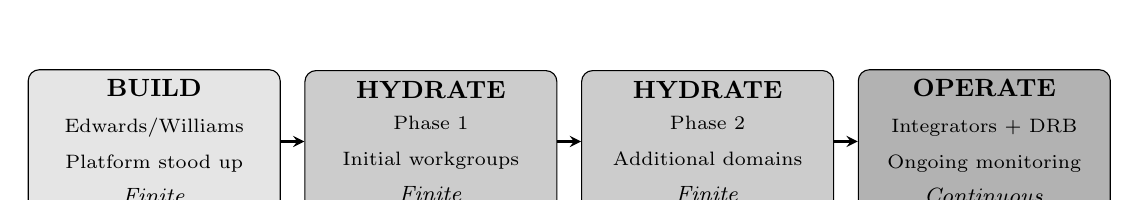
\begin{tikzpicture}[
    node distance=0.3cm,
    phase/.style={rectangle, draw, rounded corners, minimum width=3.2cm, minimum height=1.8cm, align=center, font=\small},
    arrow/.style={->, thick, >=stealth}
]
    \node[phase, fill=black!10] (build) {\textbf{BUILD}\\[2pt]{\scriptsize Edwards/Williams}\\[2pt]{\scriptsize Platform stood up}\\[2pt]{\footnotesize\textit{Finite}}};
    \node[phase, fill=black!20, right=of build] (hydrate1) {\textbf{HYDRATE}\\{\scriptsize Phase 1}\\[2pt]{\scriptsize Initial workgroups}\\[2pt]{\footnotesize\textit{Finite}}};
    \node[phase, fill=black!20, right=of hydrate1] (hydrate2) {\textbf{HYDRATE}\\{\scriptsize Phase 2}\\[2pt]{\scriptsize Additional domains}\\[2pt]{\footnotesize\textit{Finite}}};
    \node[phase, fill=black!30, right=of hydrate2] (operate) {\textbf{OPERATE}\\[2pt]{\scriptsize Integrators + DRB}\\[2pt]{\scriptsize Ongoing monitoring}\\[2pt]{\footnotesize\textit{Continuous}}};
    
    \draw[arrow] (build) -- (hydrate1);
    \draw[arrow] (hydrate1) -- (hydrate2);
    \draw[arrow] (hydrate2) -- (operate);
\end{tikzpicture}
\end{center}

\vspace{0.5em}
\begin{tabular}{@{}p{3.5cm}p{4cm}p{6cm}@{}}
\toprule
\textbf{Mode} & \textbf{Focus} & \textbf{Deliverable} \\
\midrule
\textbf{Build the Platform} & Infrastructure, tooling, architecture & Dagster+, Iceberg catalog, CDC pipelines, observability stack \\
\textbf{Hydrate the Platform} & Initial data loading, establishing flows & Bronze/Silver/Gold layers populated; source systems connected \\
\textbf{Operate} & Continuous delivery + governance & Domain-specific pipelines, new data products; DRB oversight \\
\bottomrule
\end{tabular}

\vspace{0.5em}
\noindent \textbf{Current state:} Mark Edwards and Catie Williams are chartered with building the platform. BUILD phase concludes when the platform is technically capable of receiving end-to-end data pipelines. Some disciplines (Estimating, Scheduling, Earned Value/InEight) are already ready for hydration and can begin real progress on KIP-governed data projects.

\noindent \textbf{Edwards/Williams continuing responsibilities:}
\begin{itemize}
    \item Ensure the Architecture Review Board (ARB) makes timely decisions
    \item Commission the Data Review Board (DRB) for ongoing governance
    \item Ensure InEight data—a critical, large-scale source—is successfully implemented into the platform
\end{itemize}

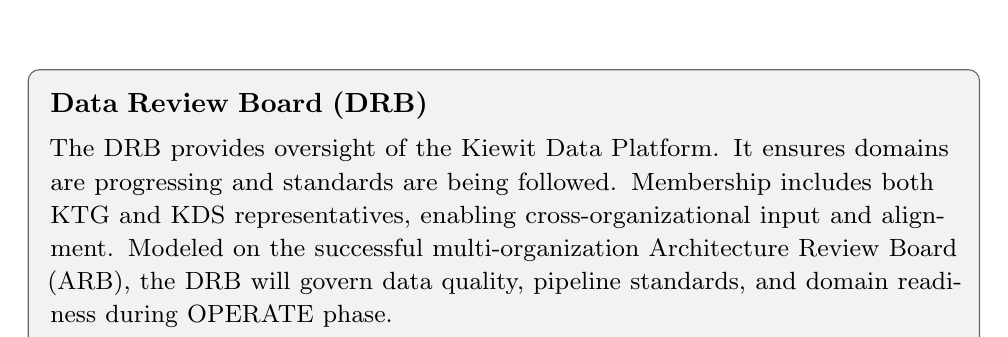
\begin{tikzpicture}
\node[draw=black!60, fill=black!5, rounded corners, inner sep=8pt, text width=0.95\textwidth] {
\textbf{Data Review Board (DRB)}\\[4pt]
{\small The DRB provides oversight of the Kiewit Data Platform. It ensures domains are progressing and standards are being followed. Membership includes both KTG and KDS representatives, enabling cross-organizational input and alignment. Modeled on the successful multi-organization Architecture Review Board (ARB), the DRB will govern data quality, pipeline standards, and domain readiness during OPERATE phase.}
};
\end{tikzpicture}

\vspace{0.5em}
\noindent \textbf{Transition plan:} Define the end state by source system. As each source is ready, the ultimate operators of KDP 2.0 assume command of the platform for their respective work groups (the spokes). Platform builders hand off to Data Platform Integrators who own ongoing operations and project delivery.

\vspace{0.5em}
\noindent \textbf{Handoff Schedule:}

\begin{tabular}{@{}p{5.5cm}p{4.5cm}p{3cm}@{}}
\toprule
\textbf{Data Workgroup} & \textbf{Manager} & \textbf{Turnover to KDS} \\
\midrule
Scheduling & Tom Gebicke & 3/26/2026* \\
Robotic Progress Capture (Buildots/FieldAI) & Matt Pappas & 3/26/2026 \\
Estimating & Nick Weindel & 4/30/2026 \\
Earned Value / InEight Components & Tom Gebicke & 5/30/2026 \\
Procurement (InEight Vendor Docs, SAP Invoices/POs) & Samantha Gorder / Ed Smith & 5/30/2026 \\
Project Data Model (CRM, TED/PI, JOR, JLAM Training) & Matt Pappas & 5/30/2026 \\
\bottomrule
\end{tabular}

{\small *Scheduling discipline is ready now.}

\vspace{0.5em}
\noindent \textbf{Phase 2 \& 3 Leadership:} Ed Smith and Matt Pappas manage the second and third phases of platform buildout. Focus remains on the data sources above; next phase planning concludes by 5/30/2026.

\subsection{Boundary with Work Groups}
Data Engineering owns the in and out of the data platform; other work groups build on it:

\begin{tabular}{@{}p{3cm}p{5cm}p{5.5cm}@{}}
\toprule
\textbf{Work Group} & \textbf{DE Provides} & \textbf{Work Group Owns} \\
\midrule
Data Science / ML & Clean, modeled data in Silver/Gold; feature pipelines & Model development, training, deployment, inference \\
Web Development & APIs to data products; documented schemas & User interfaces, application logic, UX \\
AI / GenAI & Curated datasets; MCP server integration & Agents, prompts, model selection, RAG patterns \\
Product & Data availability, SLAs, lineage documentation & Requirements, roadmap, stakeholder alignment \\
\bottomrule
\end{tabular}

\vspace{0.5em}
\noindent \textbf{The line:} DE owns data in and out of the Kiewit Data Platform, ensuring pipelines interact across domains and perform for work groups. Work groups own what they build on the platform.
\noindent \textbf{The risk:} If DE becomes a bureaucratic bottleneck, data science will build their own pipelines to avoid delay—recreating the fragmentation we're trying to eliminate. DE must deliver velocity, not process overhead. Governance is not a scapegoat for slow DE delivery—if pipelines are slow, that's a process problem to fix, not a policy to hide behind.

\section{Success Metrics}

How do we know this is working?

\begin{tabular}{@{}p{4cm}p{9.5cm}@{}}
\toprule
\textbf{Metric} & \textbf{Evidence} \\
\midrule
KDP 1.0 Decommission & Removal of legacy Snowflake objects; migration to KDP 2.0 Iceberg tables \\
Velocity Improvement & Testimonials from data workgroups/domains on faster delivery (no measured baseline—qualitative feedback) \\
Pipeline Performance & Measurable improvement in pipeline runtime, reliability, and observability vs. previous state \\
Domain Turnover & All domains turned over to KDS operators by \textbf{July 2026} (hard stop) \\
\bottomrule
\end{tabular}

\section{Risks \& Mitigations}

\begin{tabular}{@{}p{4.5cm}p{9cm}@{}}
\toprule
\textbf{Risk} & \textbf{Mitigation} \\
\midrule
InEight data delays (again) & Edwards/Williams own InEight implementation; escalation path to KIP leadership \\
DE becomes bottleneck & Velocity is a core metric; DRB monitors and intervenes \\
Governance used as excuse & Process problems are fixed, not hidden behind policy \\
Resource constraints & Phase 2 \& 3 scoped to available capacity; next phase planning by 5/30/2026 \\
\bottomrule
\end{tabular}

\section{Build Phase Completion}

BUILD phase concludes when:
\begin{enumerate}
    \item Platform is technically capable of receiving end-to-end data pipelines
    \item All domains in the Handoff Schedule are turned over to KDS operators
    \item \textbf{Not to exceed July 2026}
\end{enumerate}

\end{document}
